\subsection{Sphinx Packet Format}

HOPR uses the SPHINX packet format to encapsulate and route data packets in order to provide privacy features such as sender and receiver unlinkability.
Sphinx is a cryptographic message format used to relay anonymized messages within a mix network. A sphinx packet consists of two parts:

\begin{enumerate}
\item Header:
\begin{itemize}
\item Key derivation
\item Routing information
\item Integrity protection
\end{itemize}
\item Body:
\begin{itemize}
\item Onion-Encrypted payload
\end{itemize}
\end{enumerate}
\begin{figure}[H]
    \centering
    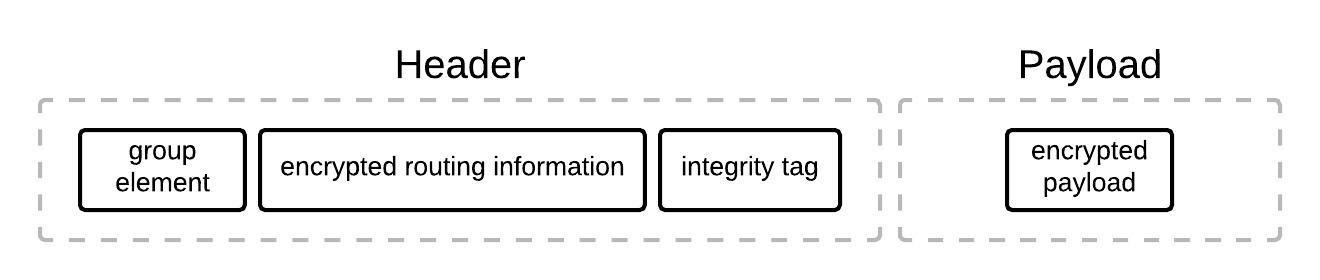
\includegraphics[width=11cm,height=11cm,keepaspectratio]{../whitepaper/images/sphinx.jpeg}
    \caption{Sphinx packet format}
    \label{fig:Sphinx packet format}
\end{figure}
\paragraph{Key derivation}
The sender (A) picks a random $x\in \mathbb{Z}^*_q$ that is used to derive new keys for every packet. 
\newline (A) randomly picks a path consisting of intermediate nodes (B), (C),(D) [see section path-finding] and the final destination of the packet (E) 
\newline (A) performs an offline Diffie-Hellman key exchange with each of these nodes and derives shared keys with each of these nodes.
\newline (A) computes a sequence of $r$ tuples (in our case r=4)  $$(a_0,s_0,b_0),.................,(a_{r-1},s_{r-1},b_{r-1})$$ as follows:
\begin{itemize}
\item $a_0=g^x,s_0=y^x_B,b_0=h(a_0,s_0)$
\item $a_1=g^{xb_0},s_1=y^{xb_0}_C,b_1=h(a_1,s_1)$
\item $a_2=g^{xb_0b_1},s_2=y^{xb_0b_1}_D,b_2=h(a_2,s_2)$
\end{itemize}
 Where $y_B,y_C,y_D,y_E$ are the public keys of the nodes $B,C, D$  which we assume are available to $A$ . The $a_i$ are the group elements which, when combined with the nodes’ public keys, allows computing a shared key for each via Diffie-Hellman key exchange, 
 and so the first node in the user-chosen route can forward the packet to the next, and only that mix-node can decrypt it.
The $s_i$ are the Diffie Hellman shared secrets, and the $b_i$ are the blinding factors.


\paragraph{Routing information}
Each node on the path needs to know the next downstream node. Therefore, the sender $(A)$ generates routing information $\beta_i$ for $(B)$, $(C)$ and (D) as well as message END to tell $(E)$ that it is the final receiver of the message. 
\newline As $(A)$ has a shared secret with each of the nodes along the path, it is able to derive blindings for each of them which is symbolised as different hatchings.
\newline Once $(B)$ receives the packet, it derives the shared key $s_0$ by computing $$s_0=(a_0)^b=(g^x)^b=(g^b)^x=y^x_B$$ and removes its blindings. This allows $(B)$ to unblind the routing info that tells $(B)$ the public key of the next downstream node $(C)$ and deletes the routing information from the packet. Afterwards, it fills the empty space with its own blinding.
\\$(B)$ also removes one layer of encryption from the payload.
Same happens at $(C)$ and $(D)$: key derivation, unblinding, deleting, shifting, decryption and blinding. 
In addition to all these steps, $(E)$ finds a message that symbolizes the end of the path and tells that it’s the recipient.

\paragraph{Integrity}
Each node along the path receives an authentication tag $\gamma_i$ in the form of a message authentication code (MAC)
 which is encoded in the header and allows to check whether or not the header was modified which guarantees integrity.










